\documentclass[a4paper, 10 pt]{article}
\usepackage{graphicx}
\usepackage{amsmath, amssymb}
\usepackage{url}
\usepackage[ruled, vlined, linesnumbered]{algorithm2e}
\usepackage{verbatim}
\usepackage{lmodern}
\usepackage[utf8]{inputenc}
\usepackage{fourier}
\usepackage{array}
\usepackage{makecell}
\usepackage{fancyhdr}
\usepackage{subfig}
\usepackage{hyperref}
\usepackage[left=2cm, right=2cm, top=2cm, bottom=2cm]{geometry}

\hypersetup{
    colorlinks=true,
    linkcolor=blue,
    filecolor=magenta,      
    urlcolor=cyan
}

\pagestyle{plain}

\title{\LARGE \bf
Hole Controlled on a 3D Map: A Physics-Based Game
}

\author{AUBERT Hippolyte Ferdinand Joseph | DE FREITAS MARTINS Alexandre Kevin \\
Department of Game Software \\
Keimyung University \\
\texttt{alexandredfm.contact@gmail.com | hippolyte.aubert@epitech.eu} \\
\href{https://github.com/AlexandreDFM/ComputerGraphics_physical_finalProject}{Github Repository}}

\begin{document}

\maketitle
\thispagestyle{plain}
\pagestyle{plain}

% --- Ideas ---
\section*{Ideas}
The core idea of our project is to create a 3D physics-based game where the player controls a mobile hole on a map. The main mechanic is inspired by games where the player grows by consuming objects in the environment. As the hole swallows more objects, it increases in size, allowing the player to interact with larger and more challenging obstacles. The goal is to combine real-time physics, interactive gameplay, and dynamic object behavior in a fun and engaging way.

% --- Features ---
\section*{Features}
\begin{itemize}
  \item \textbf{Real-time control:} Move the hole using WASD keys.
  \item \textbf{Swallowing mechanic:} Objects are pulled in and removed when overlapping the hole.
  \item \textbf{Growth system:} The hole grows in size after consuming objects, unlocking new gameplay possibilities.
  \item \textbf{Physics simulation:} Objects have variable properties (mass, collision response) and interact realistically.
  \item \textbf{Timer and score:} Track player performance with a timer and score system.
  \item \textbf{UI controls:} Buttons for running, resetting, and toggling hitbox visibility.
  \item \textbf{Hitbox visualization:} Toggle hitbox rendering for debugging and understanding collisions.
\end{itemize}

% --- Implementation ---
\section*{Implementation}
The game is implemented in C++ using OpenGL for 3D rendering and FLTK for the user interface. The physics engine is based on the Cyclone library, with custom extensions for collision detection and response. Game objects, including the hole and obstacles, are represented as 3D models with associated rigidbodies and bounding volumes.

\subsection*{Physics and Motion}
The motion of each object is governed by Newton's second law:
\begin{equation}
    \vec{F} = m \vec{a}
\end{equation}
where $\vec{F}$ is the net force, $m$ is mass, and $\vec{a}$ is acceleration. The position and velocity are updated each frame:
\begin{align}
    \vec{v}_{t+\Delta t} &= \vec{v}_t + \vec{a} \Delta t \\
    \vec{x}_{t+\Delta t} &= \vec{x}_t + \vec{v}_{t+\Delta t} \Delta t
\end{align}

\subsection*{Collision Detection}
We use Axis-Aligned Bounding Box (AABB) overlap for fast collision detection:
\begin{equation}
    \text{overlap} = (x_{1,\text{max}} > x_{2,\text{min}}) \land (x_{1,\text{min}} < x_{2,\text{max}})
\end{equation}
and similarly for $y$ and $z$ axes. For more precise collisions, the Separating Axis Theorem (SAT) is used for oriented boxes.

\subsection*{Swallowing Mechanic}
An object is swallowed if its center enters the hole's radius:
\begin{equation}
    \|\vec{x}_{\text{object}} - \vec{x}_{\text{hole}}\| < r_{\text{hole}}
\end{equation}
where $r_{\text{hole}}$ is the current radius of the hole.

\subsection*{Growth Curve}
The hole's radius increases as objects are swallowed:
\begin{equation}
    r_{\text{hole,new}} = r_{\text{hole,old}} + k \cdot m_{\text{swallowed}}
\end{equation}
where $k$ is a growth constant and $m_{\text{swallowed}}$ is the mass of the object.

The main gameplay loop handles user input, updates physics, checks for collisions, and renders the scene. The UI provides buttons to start/stop the game, reset the scene, and toggle hitbox visibility, which is useful for debugging and visualizing the physics interactions.

The codebase is organized into modular components: physics, rendering, UI, and game logic are separated for maintainability. Assets such as models and textures are loaded at runtime, and the game state is managed to allow for smooth resets and restarts.

% --- What We Learned ---
\section*{What We Learned}
This term project provided hands-on experience with real-time physics simulation, collision detection, and game development. Key takeaways include:
\begin{itemize}
  \item Integrating a physics engine with a custom rendering pipeline, and translating mathematical models into efficient code.
  \item Managing object lifecycles and dynamic scene updates, including memory management and object pooling.
  \item Designing and balancing gameplay mechanics (growth, swallowing, scoring) using mathematical formulas and playtesting.
  \item Implementing and debugging UI features, such as the hitbox toggle, to aid development and visualization.
  \item Tuning physics parameters (mass, friction, restitution) for both realism and fun, and addressing stability issues (e.g., jitter, tunneling).
  \item Working with modular code and collaborating as a team, using version control and code reviews.
  \item Gaining practical skills in C++, OpenGL, and FLTK, and learning to debug complex interactions between subsystems.
\end{itemize}

We also learned the importance of visualization tools (like hitbox rendering) for debugging and understanding the behavior of the simulation, and how small changes in parameters can have large effects on gameplay and stability.

Overall, the project deepened our understanding of interactive 3D applications and the challenges of real-time simulation and user experience design.

% --- Screenshots ---
\begin{figure*}[htbp]
    \subfloat[First Launch]{
        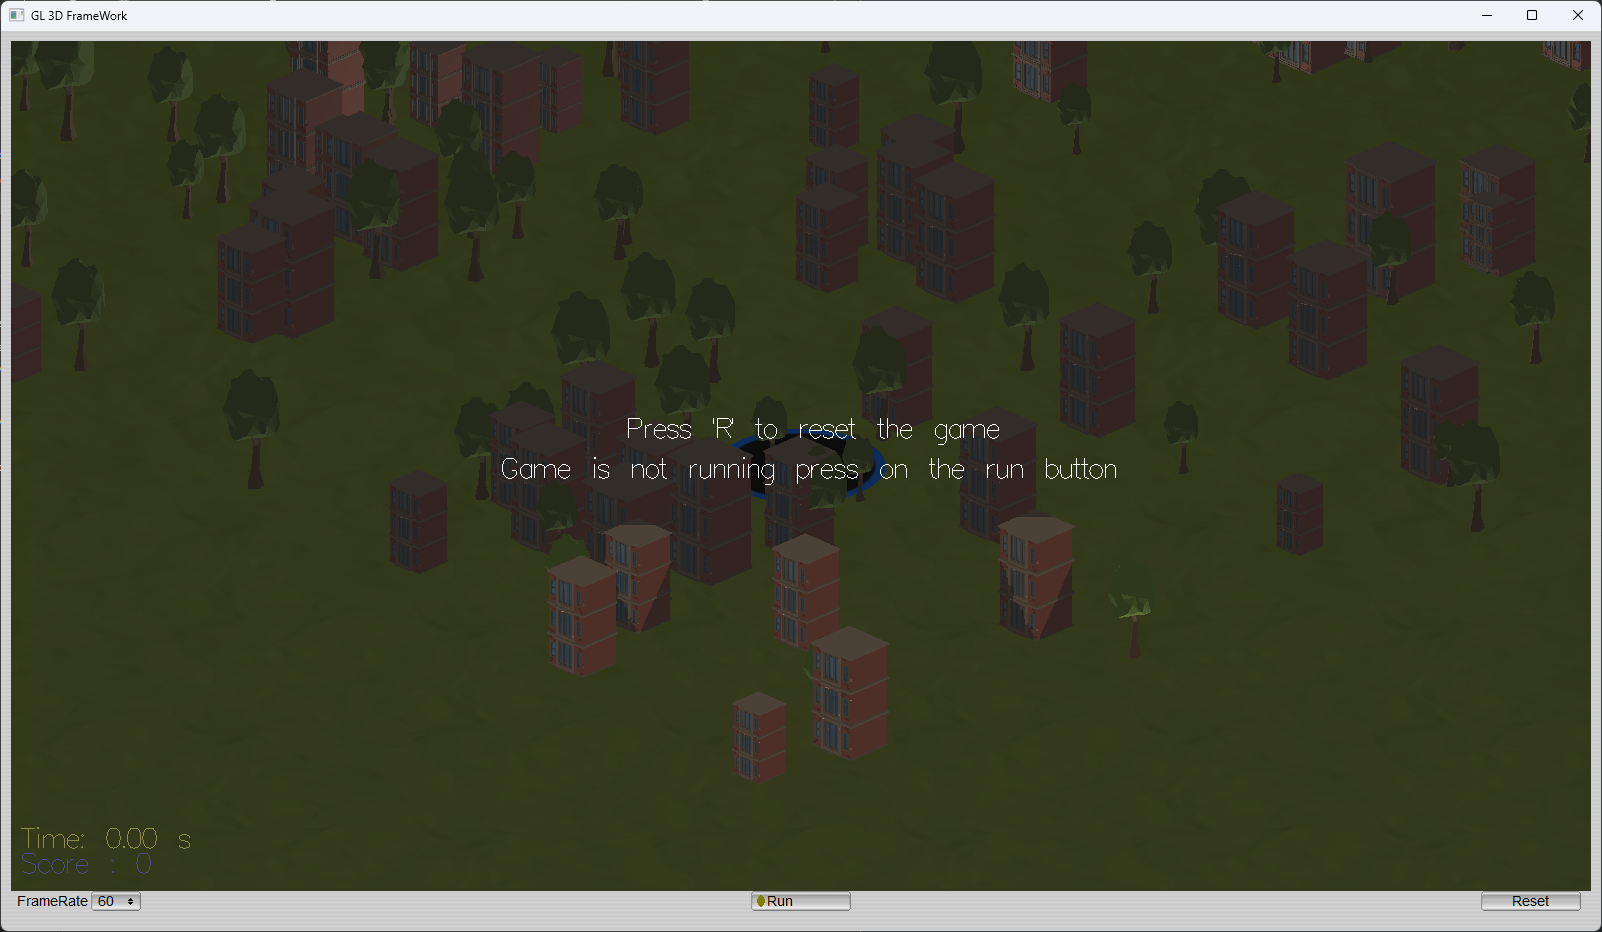
\includegraphics[width=0.48\linewidth]{assets/begin.png}
        \label{subfig:a}
    }\hfill
    \subfloat[Play Game]{
        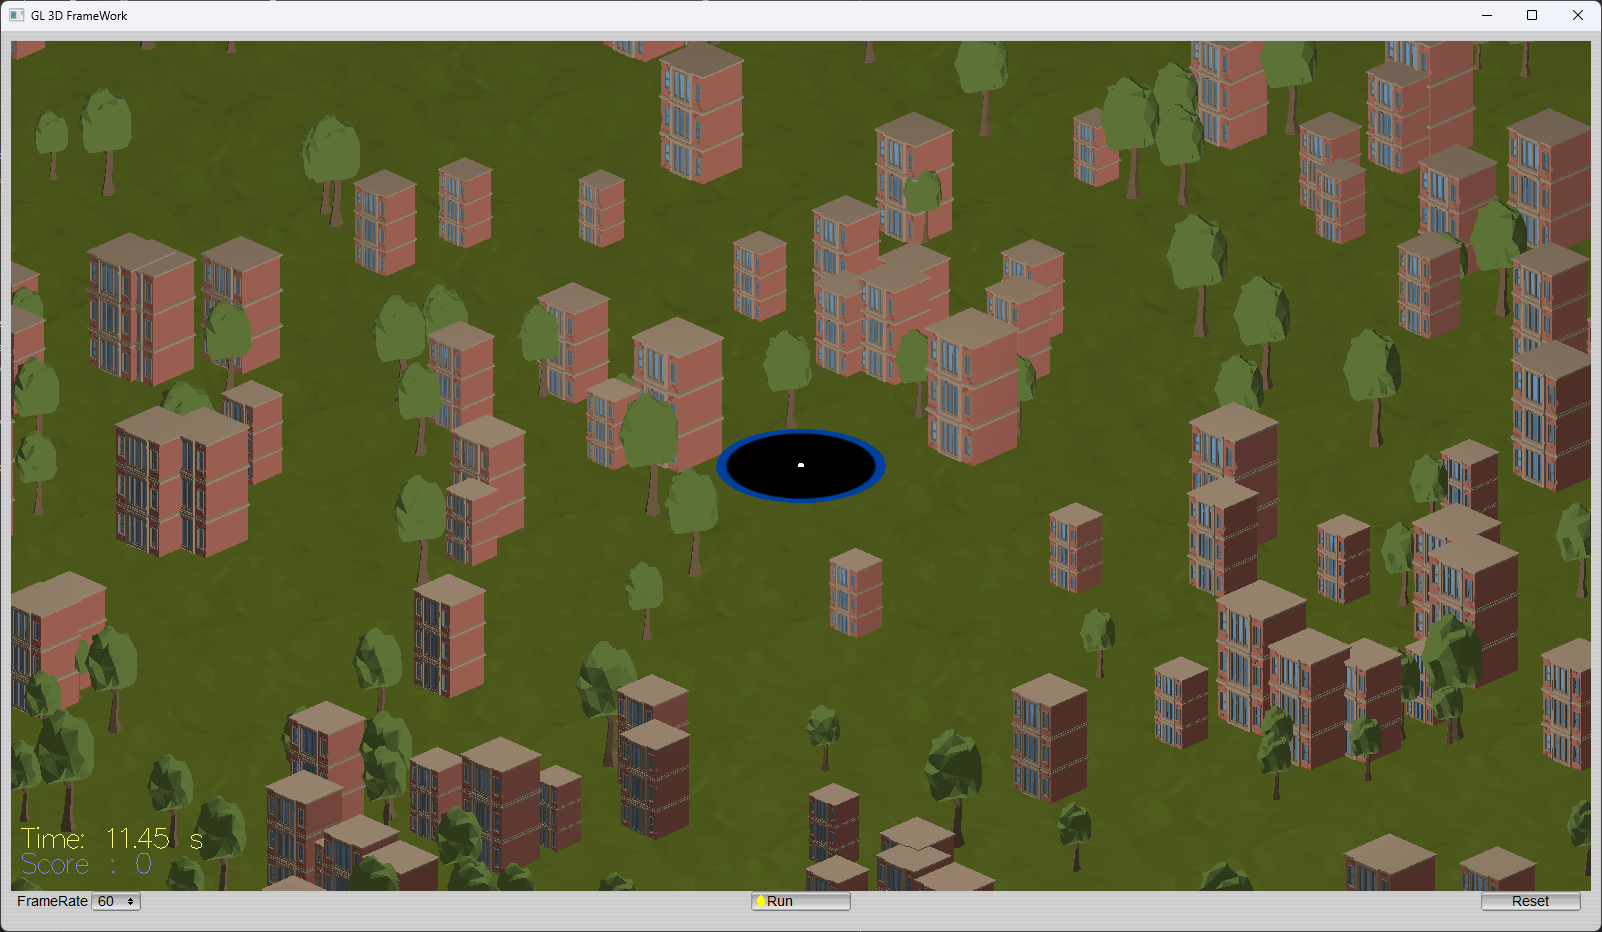
\includegraphics[width=0.48\linewidth]{assets/launch_game.png}
        \label{subfig:b}
    }
    \newline
    \subfloat[Building Swallowed]{
        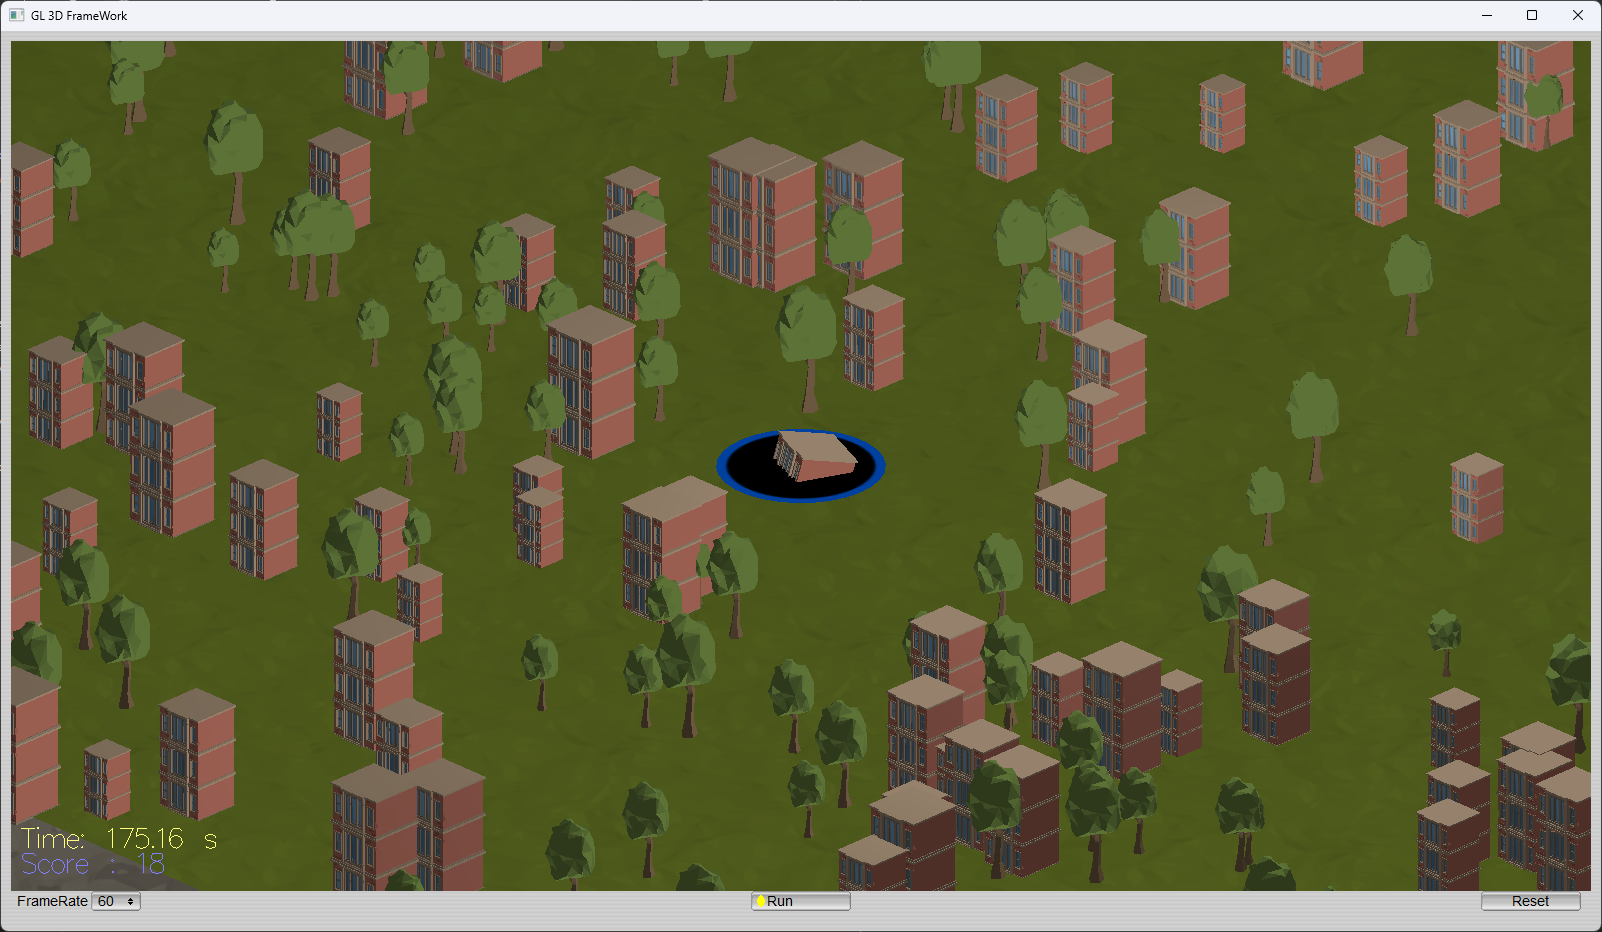
\includegraphics[width=0.48\linewidth]{assets/swallow.png}
        \label{subfig:c}
    }\hfill
    \subfloat[Hitbox Visualization]{
        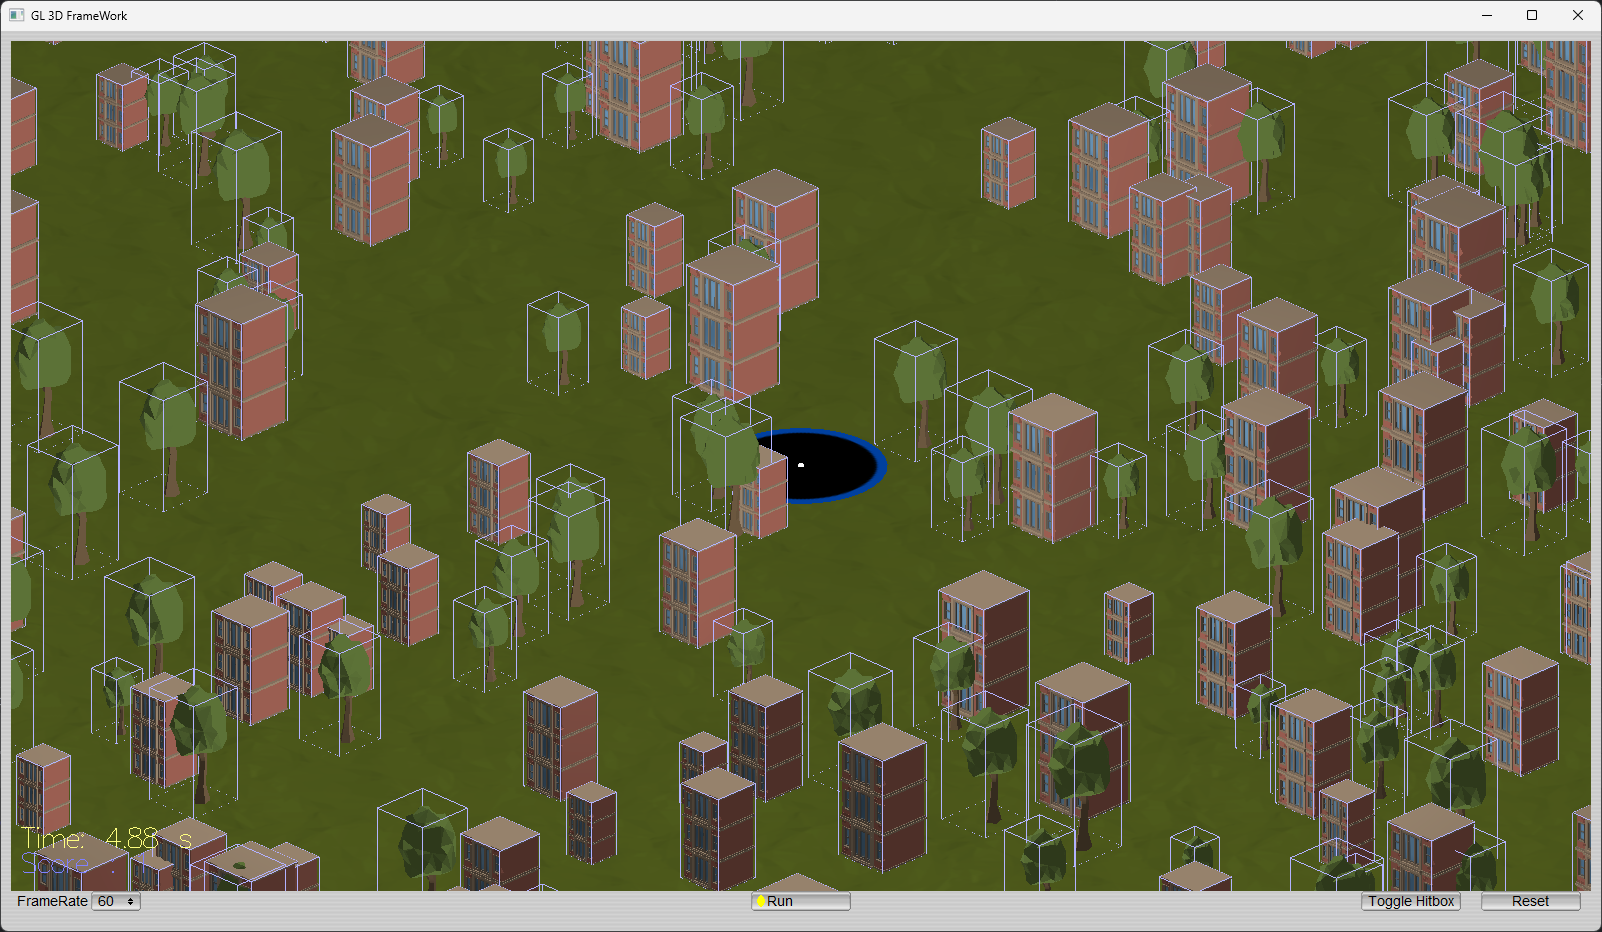
\includegraphics[width=0.48\linewidth]{assets/hitbox.png}
        \label{subfig:d}
    }
    \caption{Game Screenshots}
    \label{fig:fig}
\end{figure*}

\end{document}